\nwfilename{mainlitprog.nw}\nwbegindocs{0}\section{Introduction}% ===> this file was generated automatically by noweave --- better not edit it



We report some results on schemes in computing paths with lookahead in the stalactite and stalagmite setting. In a path with lookahead
any point on the path can see a large chunk of the path immediately ahead of it. \footnote{we are using euclidean vision where two points $A$ and $B$ see one another
iff the straight line segment $AB$ is contained in the closure of the free space. } More precisely, given a parameter $l\in \RR^{+}$ we want to compute a shortest 
path between $s$ and $t$ such that point on the computed path satisfies one of either of the two following properties


\begin{itemize}
\item The point can see at least a subpath of length $\geq l$ immediately ahead of it
\item The part of the subpath that the point can see ahead of it contains $t$
\end{itemize}

We will give a set of schemes for doing this in the alternating \textit{stalactites and stalagmites} --- henceforth shortened to ``*ites'' --- such that the shortest path 
between two given points $s$ and $t$ is taut against the tips of the ``*ites''. 



\begin{figure}[H]
\centering
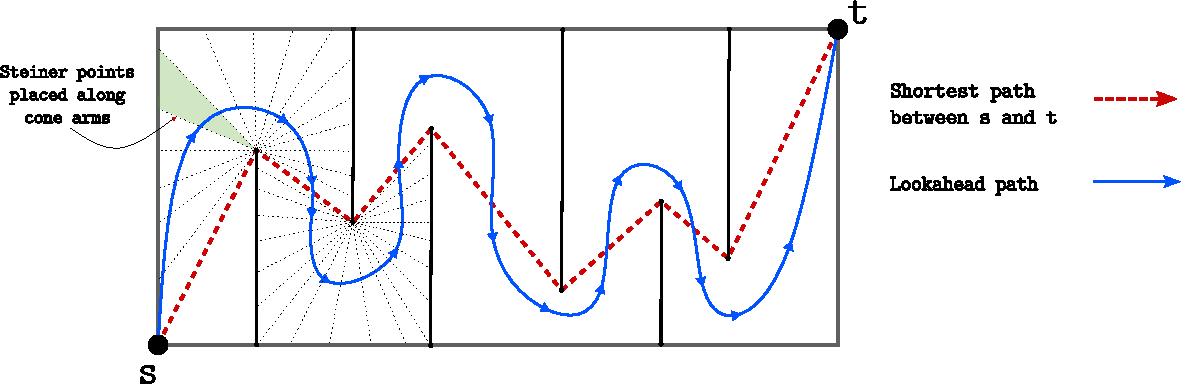
\includegraphics[width=16cm]{miscimages/stalactites-stalagmites.pdf}
\caption{Conical Routing between start $s$ and destination $t$}
\label{fig:conical-routing}
\end{figure}



\section{Basic scheme}



%%%%%%%%%%%%%%%%%%%%%%%%%%%%%%%%%%%%%%%%%%%%%%%%%%%%%%%%%%%%%%5
% Description of the rocking line setup and bipartite graph
%%%%%%%%%%%%%%%%%%%%%%%%%%%%%%%%%%%%%%%%%%%%%%%%%%%%%%%%%%%%%
\begin{figure}[H]
\centering
\begin{minipage}[t]{0.45\textwidth}
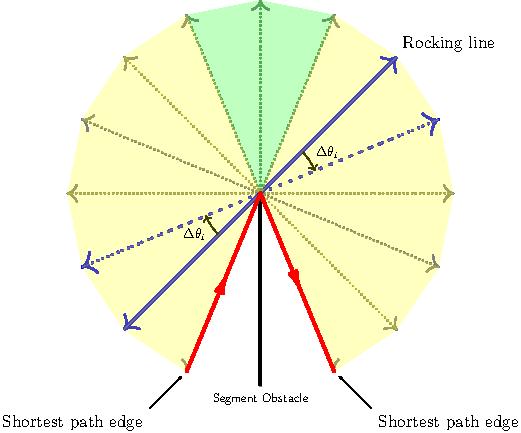
\includegraphics[width=\textwidth]{asy2d/rocking-line.pdf}
\end{minipage}
\begin{minipage}[t]{0.3\textwidth}
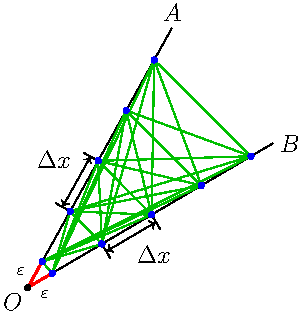
\includegraphics[width=\textwidth]{asy2d/bipartite-cone.pdf}
\end{minipage}
\caption{(Left) A rocking line (blue) creates a sequence of cones of angles 
     $\Delta \theta$ between two successive shortest path edges. (Right) Complete bipartite graph (green) between points on two arms of a cone on the Steiner points. 
              Distance between two consecutive Steiner points along each arm is $\Delta x$. $O$ is the tip of the 
      stalactite/stalagmite. See \autoref{fig:codex} for an instance of the discretization of a domain done using these rules.}
\label{fig:geomdisc}
\end{figure}




{\large \textbf{Algorithm}}

 \begin{enumerate}
  \item At each tip $T$ of the *ites, consider the two shortest path edge between $s$ and $t$ incident at that point. Divide the angle between them into 
        yellow and green wedges as shown in the left hand side \autoref{fig:geomdisc}. Each yellow wedge is divided into cones of small angle $\Delta \theta$
        whereas the green wedge is divided into small cones again of size $\Delta \theta$, allowing for one of the cones to have angle $\leq \Delta \theta$

 \item Place Steiner points separated by a small distance $\Delta x$ starting from the obstacle segment tip along each arm of every cone, 
        for as long as the cone arm lies inside free space. Also add the endpoints of the segments as Steiner points of those respective segments. 
       \footnote{computing these is just a simple matter of ray-shooting. }
 \item Draw the complete bipartite graph between the Steiner points of each cone  as shown in \autoref{fig:geomdisc}
 \item Label the cones as $C_0, C_2, \ldots C_{n-1}$ in order from the cone containing $s$ to the one containing $t$. 
       Let the first arms of each cone (as encountered in going from $s$ to $t$ be named $A_i$).
       
 \item Solve the following integer program. 
           

\begin{align}
\min \sum_{e \in E} c_e x_e  
\end{align}

such that 

\begin{align}
  x_e &\in \{0,1\} \\
  \sum_{e\in C_i} x_e &= 1  \qquad   0 \leq i \leq n-1 \label{eq:onepercone} \\ 
  \sum_{u \in A_i} x_{u,v} &= \sum_{w \in A_{i+1}}x_{v,w} \qquad \forall v \in A_i ,  \;\;\; 1\leq i \leq n-1  \label{eq:flow} \\ 
  \sum_{v \in A_0} x_{s,v} &= 1      \label{eq:sbelong}    \\   
  \sum_{u \in A_{n-1}} x_{u,t} &= 1  \label{eq:tbelong} \\
    \sum_{e\in H_{j,k}} x_{e } &\geq \ell \qquad 1\leq j \leq \lceil \frac{\Theta_k}{\Delta \theta} \rceil \label{eq:lookcons}
\end{align}
 
{\large \textbf{Notes} \normalsize}
    
\begin{itemize}
\item   \autoref{eq:onepercone} are constraints that force the choice of exactly one edge per cone. 

\item   \autoref{eq:flow} are flow constraints that make the selected set of edges form a connected path. 
     
\item   \autoref{eq:sbelong} and \autoref{eq:tbelong} force $s$ and $t$ to be terminal nodes of the computed path.   

\item   \autoref{eq:lookcons} enforces the lookahead constraint around each *ite tip, Here, $\Theta_k$ is the angle between the edges of the shortest path incident at the $k^{\text{th}}$ *ite tip
   such that the angle does not contain the *ite. Around each *ite tip there is a sequence of halfplanes. We globally label 
   these halfplanes with a 2d index set $\{j,k\}$ where $j$ refers to the rank of the half-plane within a sequence at the $k^{\text{th}}$ *ite
   tip.
\end{itemize}

 \end{enumerate}

This scheme has been implemented in Python {\tt 2.7.12} using the Python bindings of the CGAL {\tt 4.3.0-4} kernel on a Thinkpad laptop running Linux Mint. It is available 
at \url{https://github.com/gtelang/conicalrouting}. For solving linear and integer programs, I have used the PuLP 
library available at \url{https://coin-or.github.io/pulp/}. For graph algorithms I use NetworkX. 


\autoref{fig:codex1} and \autoref{fig:codex2} gives an example of the output of running the above program. The lookahead imposed on both curves is $\ell = 0.5$. 
The discretization of the domain with cones and the corresponding bipartite graphs is shown in light semi-transparent gray.
The shortest path is colored red, while the lookahead path is colored green. Note that the shortest path has been computed
using Dijkstra's algorithm in the graph. The exact shortest path between the two red nodes in the continuous domain in both cases is almost the same as the one computed here. 


\begin{figure}[H]
\centering
\begin{minipage}[t]{0.5\textwidth}
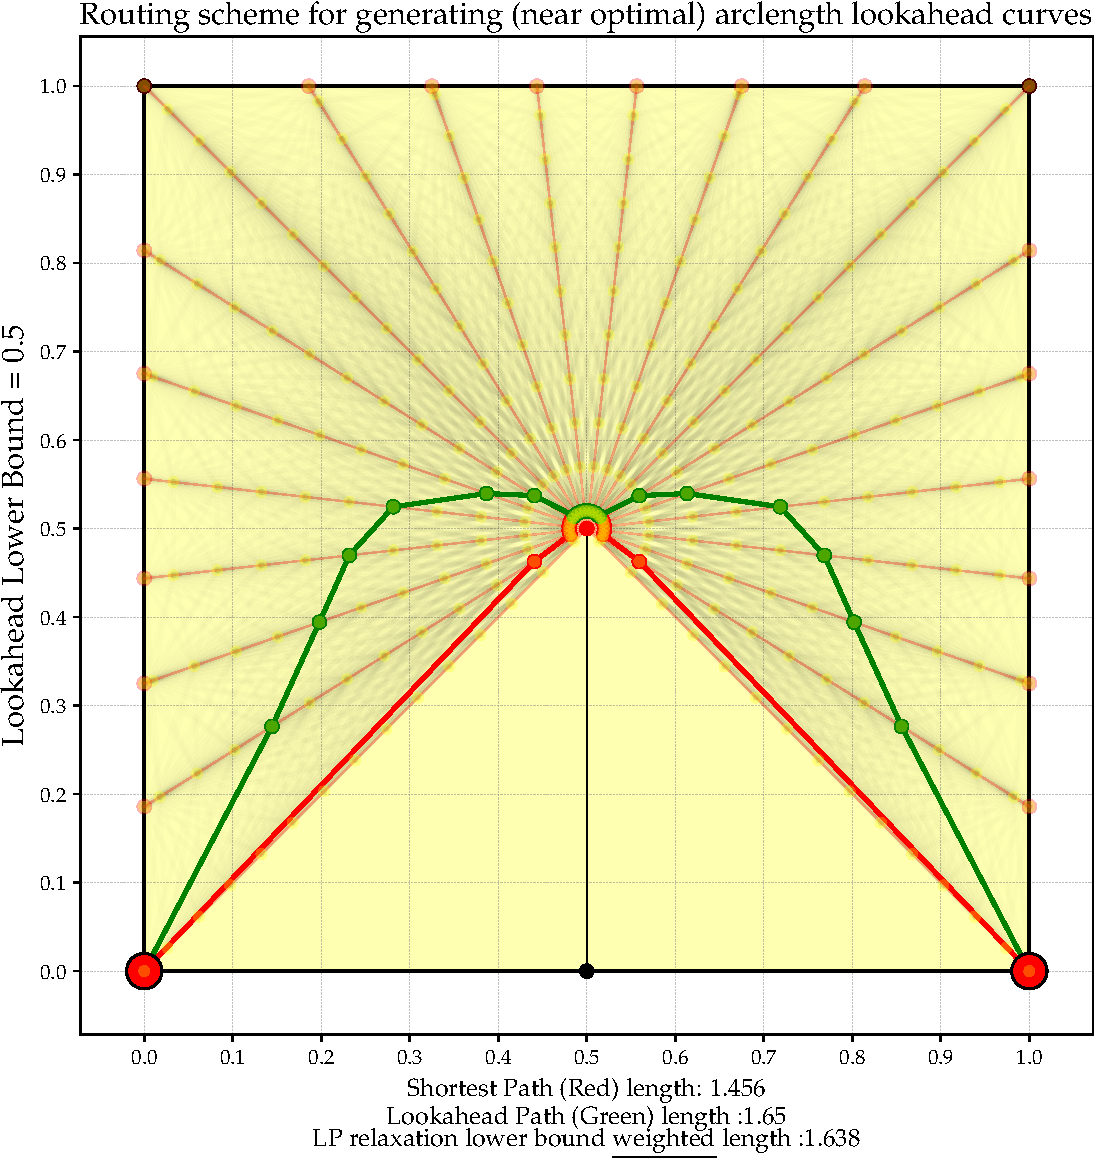
\includegraphics[width=\textwidth]{miscimages/lookex-standard.pdf}
\end{minipage}
\caption{An example of a path generated by solving the above program}
\label{fig:codex1}
\end{figure}


\begin{figure}[H]
\centering
\begin{minipage}[t]{0.5\textwidth}
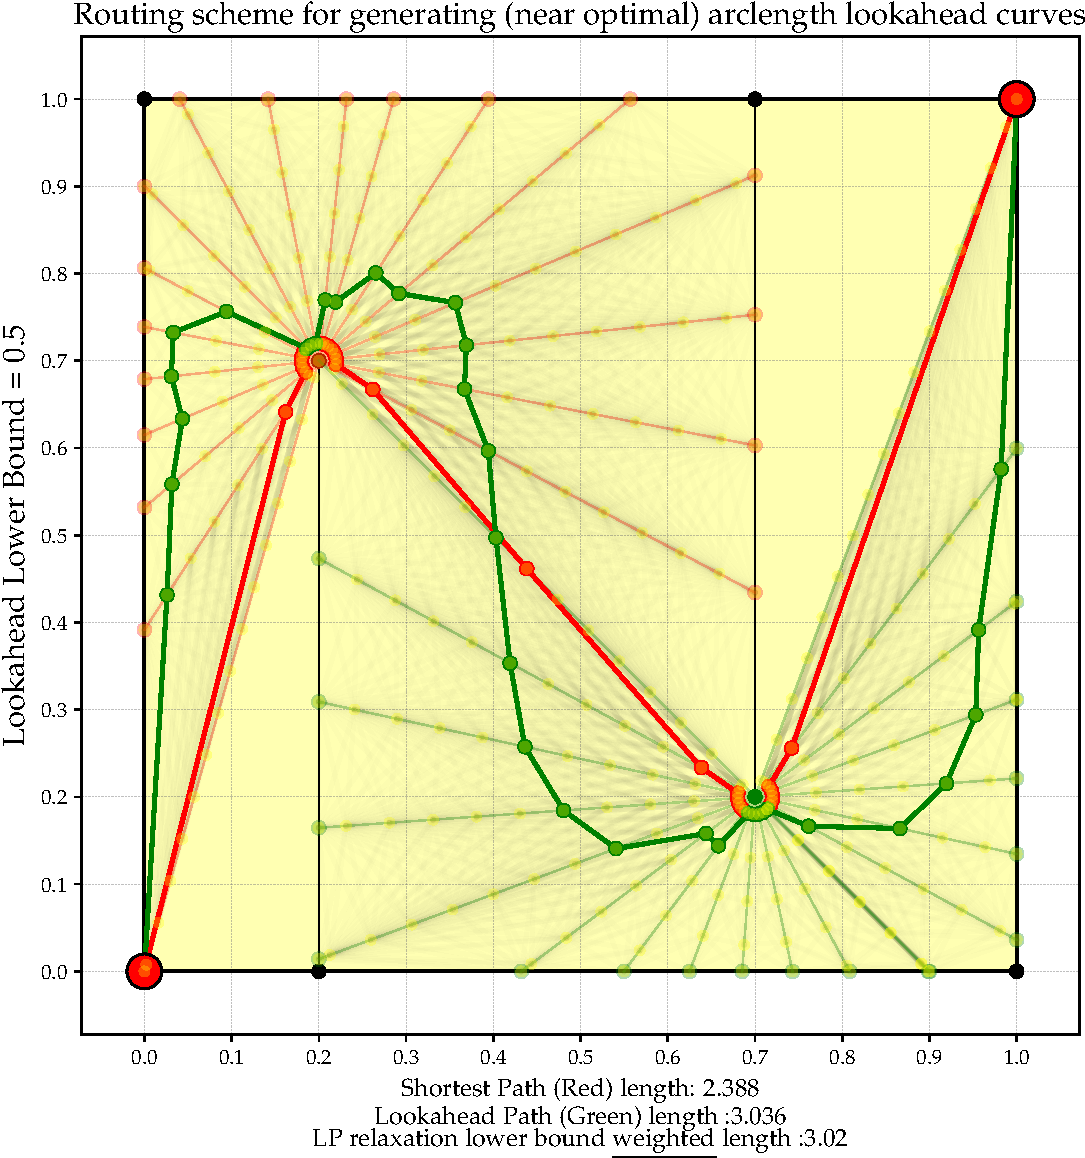
\includegraphics[width=\textwidth]{miscimages/lookex-double.pdf}
\end{minipage}
\caption{An example of a path generated by solving the above program}
\label{fig:codex2}
\end{figure}


A simple graph theoretic problem can be abstracted from this. See 
\autoref{fig:abstractmulti} 


\begin{figure}[H]
\centering
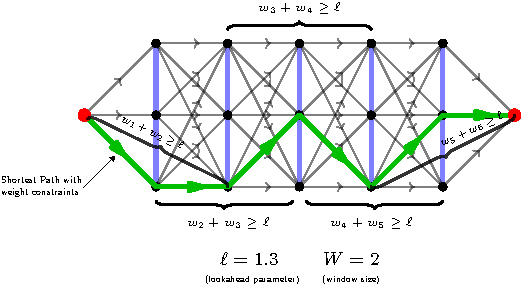
\includegraphics[width=14cm]{asy2d/multipartite-abstraction.pdf}
\caption{Instance of the $(l,W)$-multipartite lookahead problem. $W\in \NN$ is the window size and $l\in\RR^{+} \cup \{0\}$ is the 
lookahead parameter. In this problem we compute need to compute the shortest path in a weighted multipartite graph with positive edge 
weights such that the sum of consecutive $W$ edges have weight $\geq l$. The node groups of the multipartition come sequentially one 
after the other. Notice that $\ell =0$ for any $W \in \NN$ is the usual shortest path problem in such a graph.}

\label{fig:abstractmulti}
\end{figure}


\nwenddocs{}


